\documentclass[main.tex]{subfiles}

\begin{document}

\subsection{Training}

We trained classifiers to solve the problem with machine learning algorithms: Logistic Regression, Support Vector Machine, Fisher Discriminant Analysis, and Neural Networks.
For each algorithm, we check the speed of training, inference speed, and translation invariance under the same condition.
In the following sub-sections, we will describe how we used each algorithm.

\subsubsection{Logistic Regression}
Logistic Regression is designed for binary classification tasks. Given an input vector, it outputs yes or no.
Therefore, we need to adopt a heuristic, one-vs-rest, because our task is multi-class classification.
It divides multi-class dataset into several binary classification problems.
A logistic regression model is then optimized on each binary classification problem.
Finally, we use the Limited Memory BFGS (LBFGS) algorithm to optimize the model by minimizing the objective function following.

\begin{equation}
	L(\mathbf{w}, b) = \sum_{i=1}^{N} \log \left(\exp\left(-y_{i} \left(\mathbf{x}_i^{\top}\mathbf{w} + b\right)\right) + 1\right) + \frac{1}{2} \mathbf{w}^{\top}\mathbf{w}
\end{equation}


\subsubsection{Support Vector Machine}
Support Vector Machine is also a binary classifier.
Hence, we used one-vs-rest heuristic for the same reason as in logistic regression.
And we experimented with a few different kernel functions: Linear kernel, Gaussian kernel, Sigmoid kernel, and Polynomial kernel with degree 2 and 3.


\subsubsection{Fisher Discriminant Analysis}
Fisher Discriminant Analysis, unlike the previous two algorithms, allows for multi-class classification.
And it has closed-form solution rather than using iterative method.
We used least square solver to fit the model.


\subsubsection{Multi Layer Perceptron}
We design a network with the architecture following:
\begin{enumerate}[(1)]
	\item A fully connected layer to a hidden layer of size 64
	\item A rectifier non-linearity
	\item A fully connected layer to a hidden layer of size 32
	\item A rectifier non-linearity
	\item A fully connected layer that outputs a vector of size 10, corresponding to logit probabilities for each class
\end{enumerate}

The model parameters $\theta$ are updated by gradient descent using Adam optimizer on the loss function following:

\begin{equation} \label{crossentropy}
	L(\theta) = - \mathbf{t}^{\top} \log \mathbf{p} + 10^{-4} \times \|\theta\| ^2
\end{equation}


\subsubsection{Convolutional Neural Network}
Unlike other algorithms above, convolutional neural network gets the grayscale of $8 \times 8 \times 1$ itself as input without flattening.
The input data are processed by the feature extractor.

The feature extractor applies the following modules:
\begin{enumerate}[(1)]
	\item A convolutional of $16$ filters of kernel size $3 \times 3$ with stride 1 and zero-padding.
	\item A rectifier non-linearity
	\item A max-pooling of kernel size $2 \times 2$ with stride 2
	\item A convolutional of $32$ filters of kernel size $3 \times 3$ with stride 1 and zero-padding.
	\item A rectifier non-linearity
	\item A max-pooling of kernel size $2 \times 2$ with stride 2
\end{enumerate}

The output of the feature extractor is passed into a fully connected layer that outputs a vector of size 10, corresponding to logit probabilities for each class.
We optimized the model in the same way as in the case of the multi layer perceptron.

\subsection{Validation}
To measure the accuracy of each model and check whether the model is in overfitting or not, we first split the MNIST dataset into two subsets.
One is the training set. It is used to update the parameters of the models.
The other is the validation set, which consists of 200 data pairs (20 samples per class, about 11\% of the total data). It is not used to train the models directly.
Two datasets do not have any overlapped samples.

\begin{figure}[H]
	\centering
	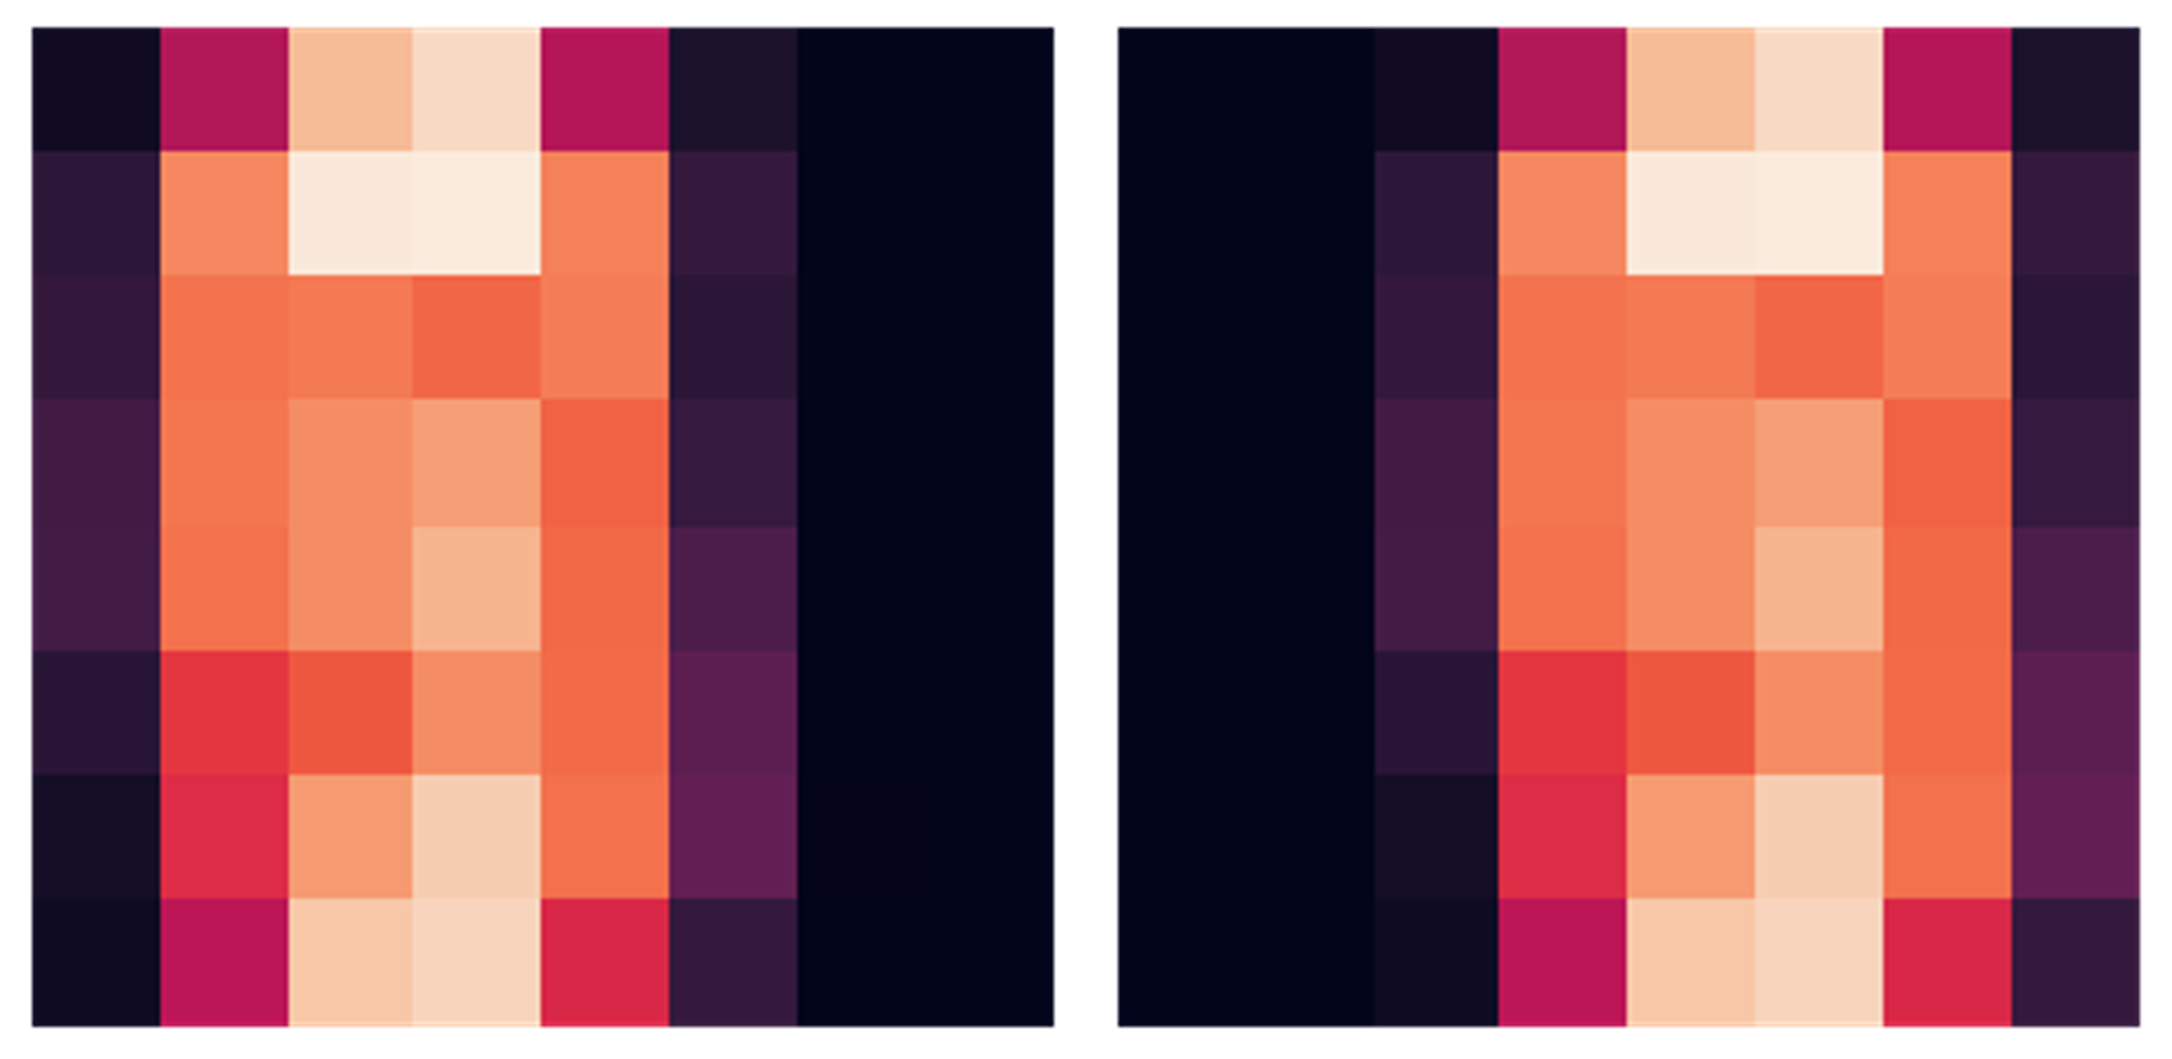
\includegraphics[scale=0.5]{img/experiment/translated_img.png}
	
	\caption{Mean image of images in translated validation set. Compared to Fig. \ref*{edafig}-(c), they are skewed to the left or right.}
	\label{translation}
\end{figure}

To test translation robustness, we also created a new validation set, translated validation dataset.
It consists of images of the validation dataset translated left or right.
It consists of a total of 400 image sets, with 200 left-biased and 200 right-biased.
However, we do not include this kind of data in the training set.
In other words, the models experience only center-centered images in the training phase.

\end{document}
